%
% parabolic.tex -- 
%
% (c) 2019 Prof Dr Andreas Mueller, Hochschule Rapperswil
%
\chapter{Parabolic partial differeential equations
\label{chapter:parabolic}}
\lhead{Parabolic partial differeential equations}
\rhead{}
In the previous chapter we were able to develop a formula for the
solution of an elliptic boundary value problem using Green's 
function.
This method depended in an essential way on the maximum principle.
It guarantees the uniqueness of solutions and thus allowed the
construction of Green's function in the first place.

For parabolic differential equations a similar technique is
available.
However, the time coordinate, i.~e.~the coordinate with 
the zero eigenvalue of the symbol matrix, will always have to be
treated specially.
We just summarize the main ideas in the first three sections
without proofs or deeper analysis.

In contrast to elliptic equations, the heat equation can also be
considered as a ``equation of motion'' for the temperature distribution
just like the ordinary differential equation $\dot x=f(x,t)$ is an
equation of motion for the state vector $x$.
The domain of the heat equation is typically of the form
$\Omega\times(0,\infty)$, where $\Omega$ is a domain in space.
The solution of the heat equation is a function in $\Omega$ with 
an additional time dependency, which we can express using a
separation ansatz.
It turns out that this allows the solution of the heat equation
by using the already established solution of the elliptic problem.

%
% problem.tex -- XXX
%
% (c) 2019 Prof Dr Andreas Mueller, Hochschule Rapperswil
%
\section{Problemstellung}
\rhead{Problemstellung}
Sei $\Omega$ ein Gebiet in $\mathbb R^n$. Der Operator 
\[
\partial_t-\kappa\Delta
\]
ist ein parabolischer Operator auf $\mathbb R_+\times \Omega$.
Eine Lösung des Wärmeleitungsproblems ist eine Funktion
$u\colon\mathbb R_+\times\Omega\to\mathbb R,$
welche folgende Bedingungen erfüllt
\begin{align*}
\partial_tu(t,x)-\kappa\Delta u(t,x)&=f(t,x)&&(t,x)\in\mathbb R_+\times\Omega
\\
u(0,x)&=u_0(x)&&x\in\Omega
\\
\alpha u+\beta\frac{\partial u}{\partial n}&=g(t, x)&&x\in\partial\Omega, t>0
\end{align*}
Falls das Gebiet $\Omega$ unbeschränkt ist, zum Beispiel $\Omega=\mathbb R^n$,
wird es notwendig sein, zusätzliche Bedingungen für das Verhalten
der Lösung für $t\to\infty$ hinzuzufügen, damit die Lösungen weiterhin
wohlbestimmt sind.


%
% minmax.tex -- XXX
%
% (c) 2019 Prof Dr Andreas Mueller, Hochschule Rapperswil
%
\section{Maximum-Minimum-Prinzip}
\index{Maximumprinzip}
\rhead{Maximum-Prinzip}
In der Theorie der elliptischen PDGL war die Mittelwerteigenschaft
der Ausgangspunkt für den Beweis des Maximumprinzips. Obwohl
diese Eigenschaft bei den 
Lösungen der Wärmeleitungsgleichung nicht mehr erfüllt ist,
gilt für sie ein Maximum-Minimum-Prinzip.
\begin{satz}[Maximum-Minimum-Prinzip für die Wärmeleitungsgleichung]
Sei $\Omega$ ein beschränktes Gebiet und
$u$ eine Funktion auf $[0,T]\times\Omega$.
Weiter sei
\begin{align*}
M_{\partial \Omega}&:=\max\{u(t,x)\,|\,x\in\partial\Omega, t\in[0,T]\}
&
m_{\partial \Omega}&:=\min\{u(t,x)\,|\,x\in\partial\Omega, t\in[0,T]\}
\\
M_0&:=
\max\{u(0,x)\,|\,x\in\Omega\}
&
m_0&:=
\min\{u(0,x)\,|\,x\in\Omega\}
\\
M&:=\max\{M_0,M_{\partial\Omega}\}
&
m&:=\min\{M_0,M_{\partial\Omega}\}
\end{align*}
Falls $u$ die homogene
Wärmeleitungsgleichung erfüllt, also $\partial_tu-\kappa\Delta u=0$,
gilt
\[
m\le u(t,x)\le M\quad\forall(t,x)\in[0,T]\times\bar\Omega.
\]
\end{satz}
Wie bei den elliptischen partiellen Differentialgleichungen folgt, dass
die das homogene Anfangs- und Randwert-Problem der Wärmeleitungsgleichung
nur eine Lösung hat.


%
% particular.tex
%
% (c) 2019 Prof Dr Andreas Mueller, Hochschule Rapperswil
%
\section{Partikuläre Lösung}
\index{partikul\äre L\ösung}
\rhead{Partikuläre Lösung}
Um das anfangs des Kapitels gestellt Problem zu lösen, kann man jetzt
gleich vorgehen wie im Fall elliptischer Randwertprobleme. Zunächst
braucht man singuläre Lösungen, also Lösungen, welche die
Wärmeleitungsgleichung mit einer $\delta$-Funktion als rechte Seite
lösen.
Man kann durch etwas mühsame Rechnung nachprüfen, dass für $0<\tau<t$
der Ausdruck
\[
\frac1{(4\pi\kappa(t-\tau))^{\frac{n}2}}
\exp\biggl(-\frac{|x-\xi|^2}{4\kappa(t-\tau)}\biggr)
\]
die Wärmeleitungsgleichung erfüllt. Daraus lässt sich
dann die Funktion
\begin{equation}
K(t-\tau, x-\xi)
=
\vartheta(t-\tau)
\frac1{(4\pi\kappa(t-\tau))^{\frac{n}2}}
\exp\biggl(-\frac{|x-\xi|^2}{4\kappa(t-\tau)}\biggr)
\label{parabolischsingulaer}
\end{equation}
konstruieren, welche die gewünschten Eigenschaften hat:

\begin{satz}
Die Funktion $K$ erfüllt die Wärmeleitungsgleichung
\begin{align*}
\partial_tK-\kappa\Delta_xK&=0&&(\tau, \xi)\ne(t,x)
\\
\lim_{t\to\tau^+}K(t-\tau, x-\xi)&=\delta(x-\xi).
\end{align*}
Bezüglich der Koordinaten $(\tau,\xi)$ gilt
\begin{align*}
-\partial_{\tau} K-\kappa\Delta_{\xi}K&=0\qquad(\tau,\xi)\ne(t,x)
\\
\lim_{\tau\to t^-}K(t-\tau, x-\xi)&=\delta(x-\xi)
\end{align*}
\end{satz}

Eine partikuläre Lösung des Problems kann wieder mit Hilfe eines Integrals
gefunden werden:
\begin{align*}
u(t,x)
&=
\int_\Omega\int_0^\infty
K(t-\tau,x-\xi)f(\tau,\xi)
\,d\tau\,d\xi
\\
&=
\int_\Omega\int_0^\infty
\vartheta(t-\tau)\frac1{(4\pi\kappa(t-\tau))^{\frac{n}2}}
\exp\biggl(-\frac{|x-\xi|^2}{4\kappa(t-\tau)}\biggr)
f(\tau,\xi)
\,d\tau\,d\xi
\\
&=
\int_\Omega\int_0^t
\frac1{(4\pi\kappa(t-\tau))^{\frac{n}2}}
\exp\biggl(-\frac{|x-\xi|^2}{4\kappa(t-\tau)}\biggr)
f(\tau,\xi)
\,d\tau\,d\xi
\end{align*}
Setzt man dies in die Wärmeleitungsgleichung ein, ergibt sich
\begin{align*}
(\partial_t-\kappa\Delta)u
&=
\int_\Omega\int_0^t
(\partial_t-\kappa\Delta)\biggl[
\frac1{(4\pi\kappa(t-\tau))^{\frac{n}2}}
\exp\biggl(-\frac{|x-\xi|^2}{4\kappa(t-\tau)}\biggr)\biggr]
f(\tau,\xi)
\,d\tau\,d\xi
\\
&\quad+
\lim_{\tau\to t-}
\int_\Omega
\frac1{(4\pi\kappa(t-\tau))^{\frac{n}2}}
\exp\biggl(-\frac{|x-\xi|^2}{4\kappa(t-\tau)}\biggr)
f(t,\xi)
\,d\xi
\end{align*}
Das erste Integral verschwindet, weil der Ausdruck in der eckigen Klammer
für alle $0<\tau<t$ die Wärmeleitungsgleichung erfüllt, also von
$\partial_t-\kappa\Delta$ zu $0$ gemacht wird.
Der Teil des Integranden vor $f(t,\xi)$ im zweiten Integral ist eine
Approximation der $\delta$-Funktion an der Stelle $x$, also ist der Grenzwert
$f(t,x)$. Insgesamt ist also
\[
(\partial_t-\kappa\Delta)u=f,
\]
wie behauptet.


%
% green.tex
%
% (c) 2019 Prof Dr Andreas Müller, Hochschule Rapperswil
%
\documentclass[tikz,12pt]{standalone}
\usepackage{amsmath}
\usepackage{times}
\usepackage{txfonts}
\usepackage{pgfplots}
\usepackage{csvsimple}
\usetikzlibrary{arrows,intersections,math}
\begin{document}
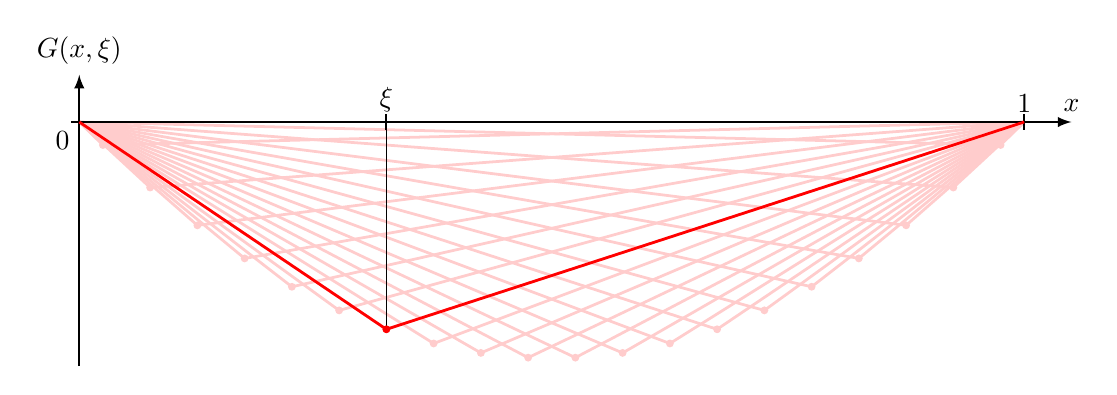
\begin{tikzpicture}[>=latex]

\def\s{12}

\foreach \xi in {0.025,0.075,...,1}{
	\draw[color=red!20,line width=1pt] (0,0)--({\s*\xi},{\s*\xi*(\xi-1)});
	\draw[color=red!20,line width=1pt] ({\s*\xi},{\s*\xi*(\xi-1)})--(\s,0);
	\fill[color=red!20] ({\s*\xi},{\s*\xi*(\xi-1)}) circle[radius=0.05];
}

\draw[->,line width=0.7pt] (-0.1,0)--({\s+0.6},0) coordinate[label=$x$];
\draw[->,line width=0.7pt] (0,{-0.25*\s-0.1})--(0,0.6)
	coordinate[label={$G(x,\xi)$}];

\draw[line width=0.7pt] ({\s},-0.1)--({\s},0.1);
\node at ({\s},0) [above] {$1$};
\node at (0,0) [below left] {$0$};

\def\xiv{0.325}

\draw[line width=0.5pt] ({\s*\xiv},0)--({\s*\xiv},{\s*\xiv*(\xiv-1)});
\draw[line width=0.7pt] ({\s*\xiv},-0.1)--({\s*\xiv},0.1);
\node at ({\s*\xiv},0) [above] {$\xi$};

\draw[color=red,line width=1pt] (0,0)--({\s*\xiv},{\s*\xiv*(\xiv-1)});
\draw[color=red,line width=1pt] ({\s*\xiv},{\s*\xiv*(\xiv-1)})--(\s,0);
\fill[color=red] ({\s*\xiv},{\s*\xiv*(\xiv-1)}) circle[radius=0.05];

\end{tikzpicture}
\end{document}


%
% causality.tex -- 
%
% (c) 2019 Prof Dr Andreas Mueller, Hochschule Rapperswil
%
\section{Causality}
The singular solution $K$ demonstrates that a change in $f$ at
$(t_0,x_0)$ affects all values of the solution $u(t,x)$ for $t>t_0$.
A disturbance at time $t_0$ propagates instantaneously throughout
the the $\Omega$.


%
% eigenfunctions.tex -- 
%
% (c) 2019 Prof Dr Andreas Mueller, Hochschule Rapperswil
%
\section{Eigenfunctions and solutions of the heat equation}
\rhead{Eigenfunctions}
In the previous chapter we have studied the problem
\begin{align*}
\Delta u&=f&&\text{in $\Omega$}\\
u&=g&&\text{on $\partial\Omega$}
\end{align*}
and found that similarly to matrix equations $Ax=b$ Green's function is a kind
of inverse.
Formally, the solution is similar to a matrix equation in the sense
that we just had to replace the sums used in matrix operations by
integrals.

For a parabolic differential equation we have to add time development.
In the framework of a matrix problem, we would have to solve the
equation $\dot x = Ax$, which can be solved by the matrix
exponential function.
The latter is most elegantly computed using eigenvectors, so the
natural questions arises whether we can solve the heat equation
using the eigenvectors of the associated elliptic problem.

This section intends to substantiate this plan.

\subsection{Systems of ordinary differential equation}
The problem analogous to a parabolic partial differential equation
is a ordinary homogeneous linear differential equation for a vector valued
function $t\mapsto x(t)\in\mathbb R^n$.
Such a system can be stated as
\[
\frac{d}{dt}x(t)=Ax(t)
\]
with some constant Matrix $A$.

If tthe matrix $A$ was diagonal, the general solution could be given
immediately as
\[
A=\begin{pmatrix}
\lambda_1&\dots&0\\
\vdots&\ddots&\vdots\\
0&\dots&\lambda_n
\end{pmatrix}
\qquad\Rightarrow\qquad
x(t)=\begin{pmatrix}
x_1(0)e^{\lambda_1t}
\\
\vdots
\\
x_n(0)e^{\lambda_nt}
\end{pmatrix}.
\]
Under certain conditions on the matrix $A$ we can find a set of
orthonormal eigenvectors $e_1,\dots,e_n$.
By using such a vector as initial condition, we get the solution
$e_ie^{\lambda_it}$.
Writing the initial condition as a linear combination
\[
x(0)=\sum_{i=1}^n(e_i \cdot x(0))e_i
\]
of these eigenvectors,
We can immediately write the solution of the differential equation
as a linear combination
\begin{equation}
x(t)=\sum_{i=1}^n
e^{\lambda_i t}
(e_i\cdot x(0))e_i
.
\label{development}
\end{equation}
of the basic solutions.
In fact, substituting this into the differential equation gives
\begin{align*}
\frac{d}{dt}x(t)&=\sum_{i=1}^n\lambda_ie^{\lambda_i t}(e_i\cdot x(0))e_i
\\
Ax(t)
&=\sum_{i=1}e^{\lambda_it}(e_i\cdot x(0))Ae_i
=\sum_{i=1}e^{\lambda_it}(e_i\cdot x(0))\lambda_i e_i
\end{align*}
So for a homogeneous differential equation, eigenvectors immediately
immediately give us the solution.

\subsection{Variation of constants}
The method of variation of constant allows to solve a inhomogeneous
differential equation of first order
\[
\frac{d}{dt}x(t)-Ax(t)=f(t),
\]
for a vector valued function $f$.
For this the constants in the general solution for the homogeneous 
equation are replaced by functions that depend on $t$:
\[
x(t)=\sum_{i=1}^nc_i(t)e^{\lambda_it}e_i.
\]
Substituting this into the differential equation gives
\begin{align*}
\sum_{i=1}^n\dot c_i(t)e^{\lambda_it}e_i
+
\sum_{i=1}^n\lambda_i c_i(t)e^{\lambda_it}e_i
-\sum_{i=1}^n\lambda_i c_i(t)e^{\lambda_it}e_i
&=
f(t)
\\
\sum_{i=1}^n\dot c_i(t)e^{\lambda_it}e_i
&=
f(t)
\end{align*}
By taking the scalar product with the eigenvectors
$e_i$, we get.
\[
\dot c_i(t)e^{\lambda_i t}=(e_i\cdot f(t)).
\]
Abbreviating the right hand side using
$f_i(t)=e_i\cdot f(t)$, turns this into
\[
c_i(t)=c_i(0)+\int_0^te^{-\lambda_i \tau}f_i(\tau)\,d\tau
\]
and the solution becomes
\begin{align*}
x(t)&=
\sum_{i=1}^n
(e_i\cdot x(0))e_i+
\sum_{i=1}^ne^{\lambda_i t}\int_0^te^{-\lambda_i \tau}(e_i\cdot f(\tau))e_i\,d\tau
\\
&=
x(0)
+
\int_0^t
\biggl(
\sum_{i=1}^n
e^{\lambda_i(t- \tau)}(e_i\cdot f(\tau))\biggr)e_i\,d\tau
\end{align*}
One can verify this directly:
\begin{align*}
\frac{d}{dt}x(t)
&=
\sum_{i=1}^n\left.e^{-\lambda_i (t-\tau)}(e_i\cdot f(\tau))e_i \right|_{\tau=t}
\\
&=
\sum_{i=1}^n(e_i\cdot f(t))e_i=f(t)
\end{align*}

\subsection{Eigenvalues and eigenvectors}
Assume now that the domain $\Omega$ is bounded and does not have a 
boundary too complicated, so that there is a sequence of eigenfunctions
$u_i(x)$ of the Laplace operator with eigenvalue $\lambda_i$
with homogeneous boundary conditions, i.~e.
\[
\Delta u_i=\lambda_iu_i,\qquad u_{i|\partial\Omega} = 0.
\]
In addition, we can scale these solutions so that the have 
$L^2$-norm $1$:
\[
\int_{\Omega}|u_i(\xi)|^2\,d\xi=1
\]
The general theory even guarantees that the are orthogonal:
\[
\int_{\Omega}u_i(\xi)u_j(\xi)\,d\xi=0\qquad\forall i\ne j.
\]

We now use these functions in a separation ansatz
$u(x,t)=u_i(x)\cdot T(t)$ for the parabolic equation
\[
\partial_tu=\kappa\Delta u,
\]
and get the equation
\begin{align*}
\partial_t (T(t)u_i(t))-\kappa\Delta(T(t)u_i(t))&=0
\\
T'(t)u_i(t)-\kappa T(t)\Delta u_i(t)&=0
\\
T'(t)u_i(t)-\kappa T(t)\lambda_i u_i(t)&=0
\\
\frac{T'(t)}{T(t)}&=\kappa\lambda_i
\\
\Rightarrow\qquad T(t)=Ce^{\kappa\lambda_it}
\end{align*}
In particular, for initial conditions that are eigenvalues we
immediately get a solution for the parabolic problem.

\subsection{The inhomogeous equation}
The process of variation of constants cann also be used for partial
differential equations.
We write the solution as
\[
u(t,x)=\sum_{i=0}^\infty c_i(t) e^{\kappa\lambda_i t}u_i(x)
\]
and substitute into the differential equation
\begin{align*}
\sum_{i=0}^\infty \dot c_i(t)e^{\kappa\lambda_it}u_i(x)
+\kappa\sum_{i=0}^\infty c_i(t)\kappa\lambda_i e^{\lambda_it}u_i(x)
-\kappa\sum_{i=0}^\infty c_i(t)e^{\kappa\lambda_it}\lambda_iu_i(x)
&=f(x)
\\
\sum_{i=0}^\infty \dot c_i(t)e^{\kappa\lambda_it}u_i(x)
&=f(t,x)
\end{align*}
The scalar product with $u_i$ then gives
\begin{align*}
\dot c_i(t)&= e^{-\kappa\lambda_it}\int_{\Omega}u_i(\xi)f(t,\xi)\,d\xi
\\
c_i(t)&=c_i(0)+\int_0^te^{-\kappa\lambda_i\tau}\int_{\Omega}u_i(\xi)f(\tau,\xi)\,d\xi\,d\tau
\end{align*}
and the particular solution
\begin{align*}
u(t,x)&=
\sum_{i=0}^\infty
u_i(x)
\int_0^t
e^{\kappa\lambda_i(t-\tau)}\int_{\Omega}u_i(\xi)f(\tau,\xi)\,d\xi\,d\tau
\end{align*}
Green's function for the heat equation with Dirichlet boundary conditions
can thus be written as
\[
G(t,x,\tau,\xi)
=
\sum_{i=0}^\infty
e^{\kappa\lambda_i (t-\tau)}
u_i(x)
u_i(\xi).
\]
So we have reduced the solution of the parabolic problem to the
elliptic problem.



